% 图 83.2 —— **结构化重画**（2026-09-25，替换掉 `checks/emit_hand.py` 的逐段拟合稿）
%%
% 结构：一点向外发散 4 条直线 + 顶点圆角方点 + 下方 3 个小圆点（**无文字无箭头**）
%%
% 旧版是**描摹**：把每一段笔画单独拟合后发出来，连「箭头头」都被当成"一条很粗的短线"描
%   （图 81.5 上一度出现 `\draw[line width=7.0pt] (586,277)--(586,270);` 这种 7px 长的疙瘩），
%   渲染出来是黑疙瘩而不是箭头。本版改成**看懂结构后用 TikZ 画**。
%%
% 做法、约定、已踩过的坑 → `＜工作区＞\checks\redraw\README_重画流程.md`
% 本图圆/椭圆的中心与半径、标签的文字与位置，沿用 probe 的脚手架（那部分它是对的）。
%%
% ⚠ 本图 tikzpicture 是 y=-1pt（**y 翻转**）⇒ `arc` 的角向"递减"才是屏幕逆时针；
%   同一根线上的多段弧必须同向。改完务必拿原书并排、放大核箭头朝向。
%%
\documentclass[12pt]{standalone}
\usepackage{fontspec}
\setsansfont{Arial}
\newfontfamily\mfallback{DejaVu Sans}
\usepackage{tikz}
\usetikzlibrary{arrows.meta}
\begin{document}
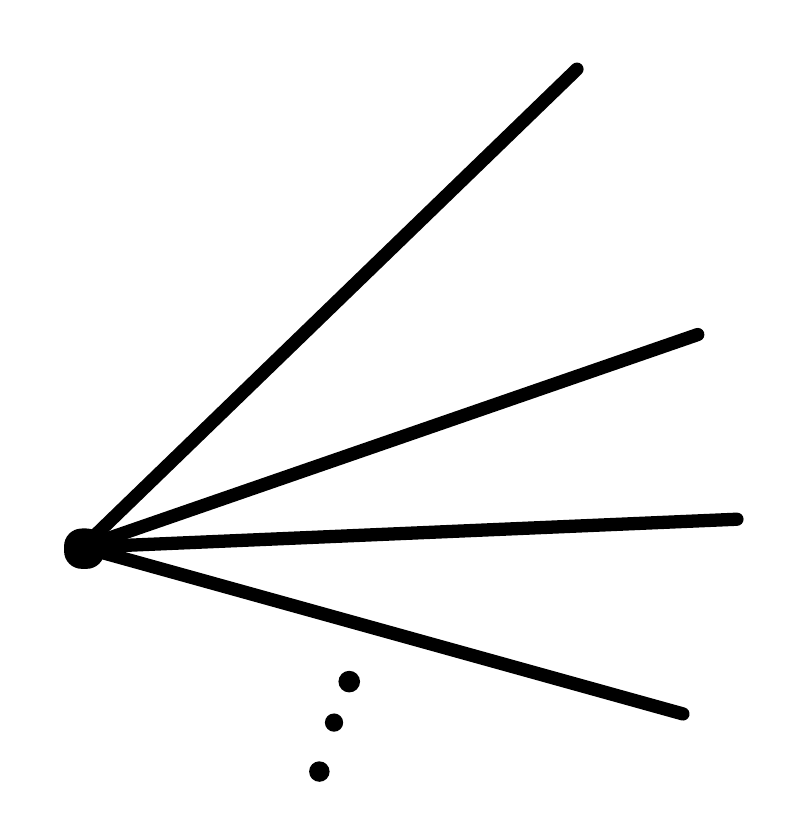
\begin{tikzpicture}[x=1pt, y=-1pt, line width=4.8pt, line cap=round, line join=round]

  % ── 扇形线束的公共端点（四线 LS 拟合的共点）──
  \coordinate (O) at (19.97,187.72);

  % ── 4 条从 O 向外发散的直线（外端 = 墨迹尖端沿 u 内收 2.4）──
  \draw (O) -- (198.48, 14.99);   % -44.06°
  \draw (O) -- (242.13,110.89);   % -19.08°
  \draw (O) -- (256.28,177.62);   %  -2.45°
  \draw (O) -- (236.76,247.97);   % +15.53°

  % ── O 处的实心大圆点（中心 (20.44,188.26)、半边长 7.29、圆角 6.40）──
  \fill[rounded corners=6.40pt] (13.15,180.97) rectangle (27.73,195.55);

  % ── 下方 3 个小实心点 ──
  \fill (116.2,236.3) circle (3.9);
  \fill (110.7,251.1) circle (3.3);
  \fill (105.4,268.8) circle (3.7);

  % 钉死画布：否则超出的图元/控制点会把页面撑大，1:1 回比就失准
  \pgfresetboundingbox
  \path[use as bounding box] (0,0) rectangle (265,279);
\end{tikzpicture}
\end{document}
